\section{Estimation of Sources of Fake and Non-prompt Leptons}
\label{sec:fakes}

Despite both the high levels of accuracy achieved by the ATLAS simulation
infrastructure and the lepton reconstruction and identification algorithms
described in Chapter~\ref{chap:objects}, sources of misidentified reconstructed
leptons still exist and lead to an additional source of backgrounds to
the analyses discussed in Chapters~\ref{chap:search_stop} and \ref{chap:search_hh}.
These background sources of leptons are broken down into two categories:
\begin{itemize}
    \item \textbf{Fake leptons}: Cases in which signals in the ATLAS detector
        are selected as being leptons when in fact there is no real lepton present
    \item \textbf{Non-prompt leptons}: When real, genuine leptons are identified
        but they are not leptons originating from the primary $pp$ hard-scatter interaction process
        of interest
\end{itemize}
In the subsequent discussion, the term `fake' will be used in reference to the two
categories listed above, unless specified otherwise.

The contribution of backgrounds leading to sources of fake leptons are generally predicted
using methods based on the observed data --- referred to as `data-driven' methods ---
and arise from various sources and mechanisms.
The sources of fake leptons will be described in Section~\ref{sec:fake_lepton_sources}, separately for
electrons and muons.
Section~\ref{sec:fake_dd_motivation} provides some reasoning for why a data-driven
approach is generally taken for estimating these backgrounds.
Sections~\ref{sec:matrix_method} and \ref{sec:same_sign_extrap} go on to describe
the two data-driven approaches taken in the analyses to be presented in this thesis
for estimating fake lepton contributions: the so-called `Matrix Method' and the `Same-sign Extrapolation Method', respectively.

%%%%%%%%%%%%%%%%%%%%%%%%%%%%%%%%%%%%%%%%%%%%%%%%%%%%%%%%%%%%%%%%%%%
%%%%%%%%%%%%%%%%%%%%%%%%%%%%%%%%%%%%%%%%%%%%%%%%%%%%%%%%%%%%%%%%%%%
%
% SOURCES OF FAKE LEPTONS
%
%%%%%%%%%%%%%%%%%%%%%%%%%%%%%%%%%%%%%%%%%%%%%%%%%%%%%%%%%%%%%%%%%%%
%%%%%%%%%%%%%%%%%%%%%%%%%%%%%%%%%%%%%%%%%%%%%%%%%%%%%%%%%%%%%%%%%%%
\subsection{Sources of Fake Leptons}
\label{sec:fake_lepton_sources}

The types and sources of fake leptons generally have different experimental signatures
than those leptons that genuinely originate from the $pp$ hard-scatter.
However, due to the non-perfect lepton identification and isolation algorithms,
such sources are able to contaminate the various regions of an analysis.
The rates of contamination are generally quite low for the analyses to be presented, but their inclusion in the background
estimates of the analyses has measurable consequences nevertheless.

The analyses to be presented in the current thesis make use of $b$-tagging algorithms
to identify jets originating from $b$-hadrons.
Fake leptons, both electrons and muons, can originate from the semi-leptonic decays of
$b$- and $c$-quarks within these $b$-tagged jets, following $b\rightarrow \ell$ or cascade-type
$b \rightarrow c \rightarrow \ell$ decays of the $B$ hadrons within the jets.
The leptons resulting from such decays are typically embedded within or very close to
the originating reconstructed jet object and the lepton isolation requirements
are intended to reduce this type of background.
The subsequent paragraphs will describe additional sources of fake electrons
and muons, which generally differ between the two lepton species.

%%%%%%%%%%%%%%%%%%%%%%%%%%%%%%%%%%%%%%%%%%%%%%%%%%%%%%%%%%%%%%%%%%%
%%%%%%%%%%%%%%%%%%%%%%%%%%%%%%%%%%%%%%%%%%%%%%%%%%%%%%%%%%%%%%%%%%%
%
% SOURCES OF FAKE ELECTRONS
%
%%%%%%%%%%%%%%%%%%%%%%%%%%%%%%%%%%%%%%%%%%%%%%%%%%%%%%%%%%%%%%%%%%%
%%%%%%%%%%%%%%%%%%%%%%%%%%%%%%%%%%%%%%%%%%%%%%%%%%%%%%%%%%%%%%%%%%%
\subsubsection{Sources of Fake Electrons}
\label{sec:fake_electron_sources}

As described in Section~\ref{sec:electrons}, electrons are reconstructed based
on the presence of well-reconstructed tracks in the ID matched to deposited
energy clusters in the EM calorimeter.
Light-flavor jets, originating from the production of light quarks ($u$, $d$, $s$),
or gluon jets, which are associated with a large number of tracks due to their
increased radiation pattern, are able to fake electrons as they leave
tracks in the ID as well as subsequent energy depositions in both the EM and hadronic calorimeters.
This background, due to mis-identified jets, is typically suppressed by the use
of lepton isolation and by jet shower-shape information used in the electron identification: the
hadronic shower shapes and radial extent differ with respect to the electromagnetic shower
produced by a genuine electron.

An additional large source of fake electrons is due to photon conversion processes,
$\gamma \rightarrow e^+ e^-$, and other electromagnetic scattering processes
that happen as a result of detector material interactions.
These processes leave both tracks in the ID and electromagnetic energy depositions
in the EM calorimeter which are difficult to distinguish from genuine electrons.
Neutral hadron decays, such as the $\pi^0 \rightarrow e^+ e^- \gamma$ Dalitz decay,
also lead to electron-like signatures.
This decay of the $\pi^0$ only has a branching fraction of just over $1\%$~\cite{PDGRef}, but given
the large production of $\pi^0$ states in the $pp$ collision this has the potential to be
a relevant source of fake electrons.
These electromagnetic sources of fake electrons are distinguished by their generally
larger impact parameters relative to genuine prompt electrons.

\begin{figure}[!htb]
    \begin{center}
        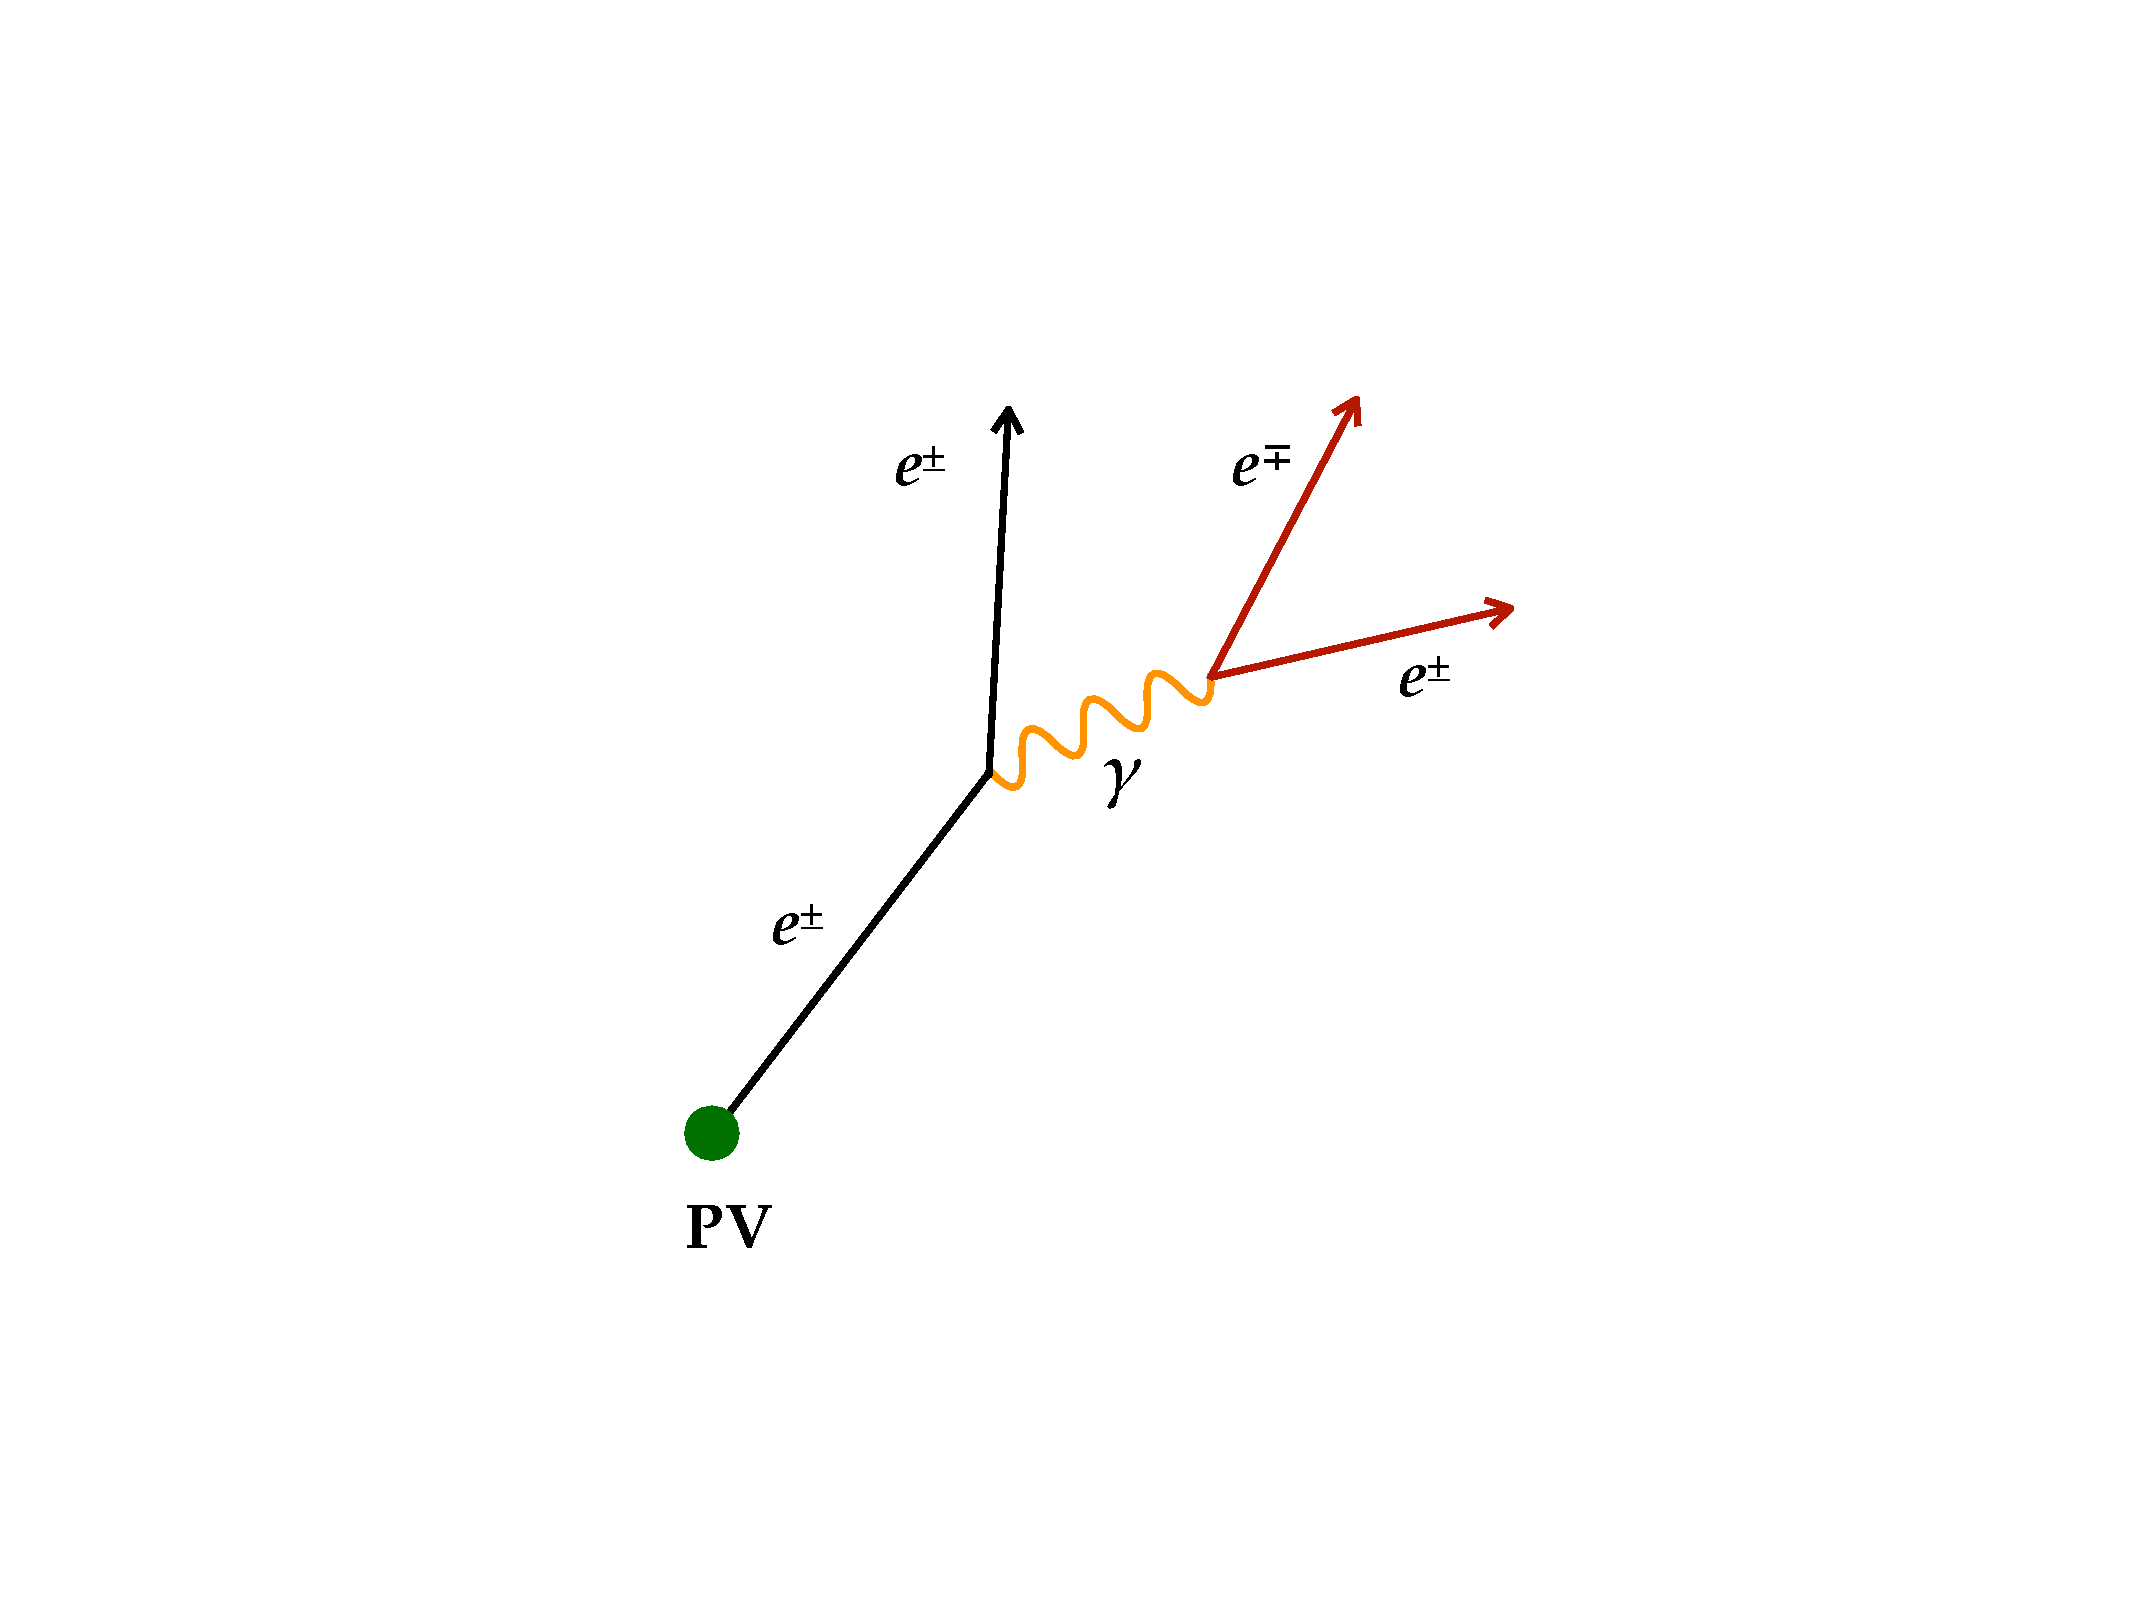
\includegraphics[width=0.45\textwidth]{figures/common_ana/fakes/electron_brem_fake}
        \caption{
        }
        \label{fig:electron_brem_fake}
    \end{center}
\end{figure}


%%%%%%%%%%%%%%%%%%%%%%%%%%%%%%%%%%%%%%%%%%%%%%%%%%%%%%%%%%%%%%%%%%%
%%%%%%%%%%%%%%%%%%%%%%%%%%%%%%%%%%%%%%%%%%%%%%%%%%%%%%%%%%%%%%%%%%%
%
% SOURCES OF FAKE MUONS
%
%%%%%%%%%%%%%%%%%%%%%%%%%%%%%%%%%%%%%%%%%%%%%%%%%%%%%%%%%%%%%%%%%%%
%%%%%%%%%%%%%%%%%%%%%%%%%%%%%%%%%%%%%%%%%%%%%%%%%%%%%%%%%%%%%%%%%%%
\subsubsection{Sources of Fake Muons}
\label{sec:fake_muon_sources}

As described in Section~\ref{sec:muons}, muons are primarily reconstructed via the combination
of tracking information provided by the ID and MS, and, generally speaking, they should be the only particle species to reach
the MS.
In addition to the semi-leptonic decays of heavy-flavored jets described above, however,
there are several sources of fake muons.
Highly energetic jets can have elongated shower profiles that reach the outer
radii of the hadronic calorimeter, with a non-zero chance of exiting the calorimeter
and resulting in particle leakage into the MS.
Such cases are referred to as calorimeter punch-through, and have been illustrated
in Figure~\ref{fig:jet_punch_through}.
Punch-through particles can leave signatures similar to charged muons whose subsequent
MS tracks are associated with a track in the ID, leading to a reconstructed combined muon
faking a genuine muon.
An additional source of fake muons come from the in-flight decays of charged hadrons,
such as the $K^\pm$ and $\pi^{\pm}$, that can decay to $\mu^{\pm} \nu$.
These sources of non-prompt muons typically result in low-\pT~muons and are characterised
by combined tracks with exhibiting a kink topology,
briefly mentioned when discussing the muon combined reconstruction in Section~\ref{sec:muon_id}.
The \pT~dependence of muon cross-sections for various sources of muons (prompt, fake, and non-prompt)
is shown in Figure~\ref{fig:fake_muon_kink}, along with an illustration of the kinked-track topology
characterising the in-flight decays of Kaons and charged pions.

\begin{figure}[!htb]
    \begin{center}
        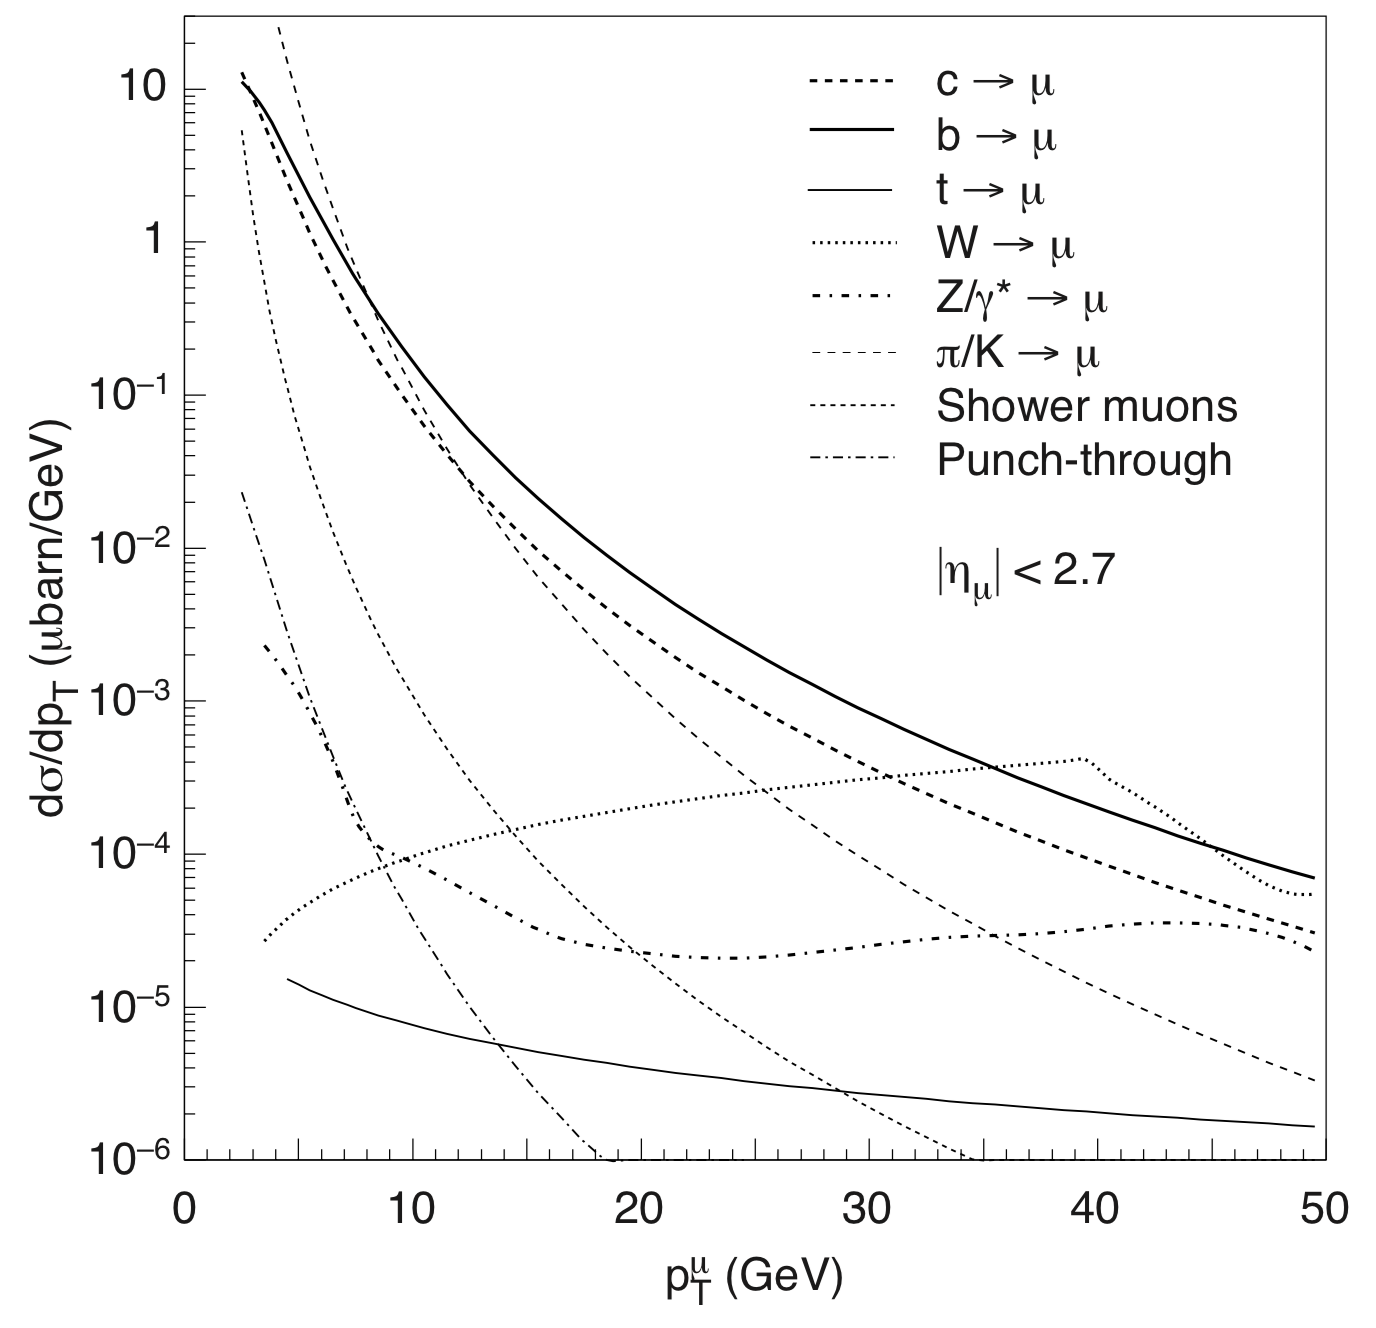
\includegraphics[width=0.43\textwidth]{figures/common_ana/fakes/reco_muon_sources}
        \raisebox{0.45cm}{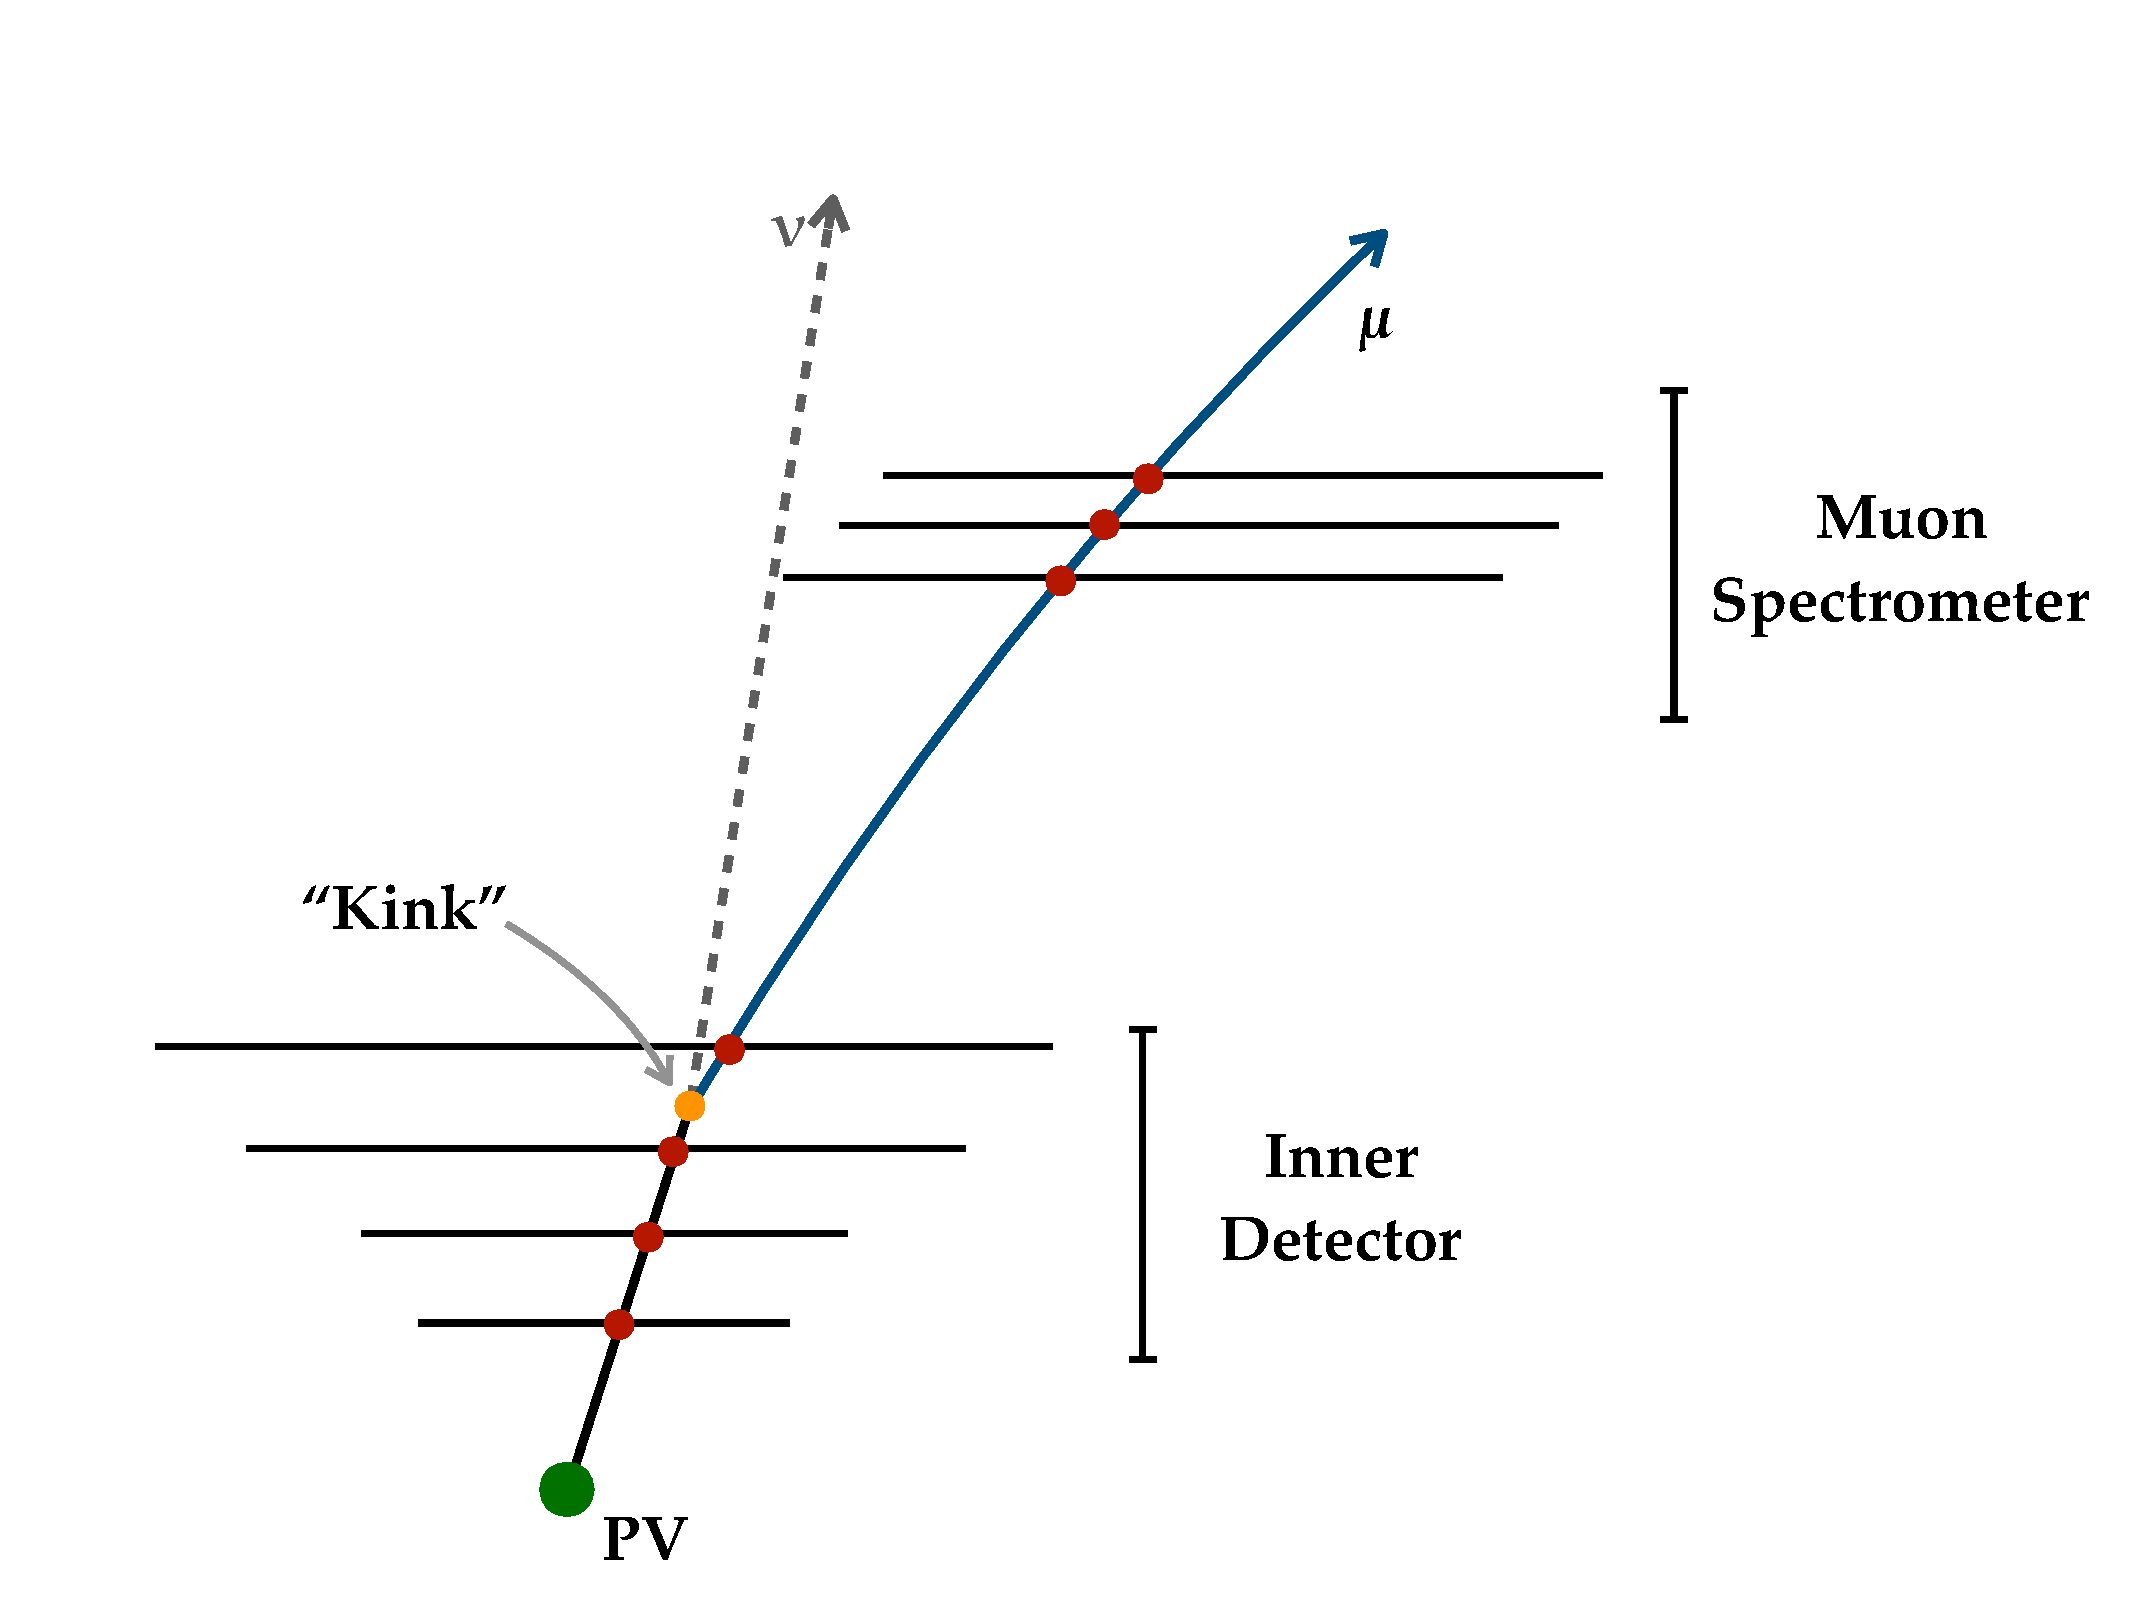
\includegraphics[width=0.54\textwidth]{figures/common_ana/fake_muon_kinkPDF}}
        \caption{
            \textbf{\textit{Left}}:  Transverse momentum dependence of muon cross-sections for muons originating
                from various prompt and non-prompt sources.
                Figure taken from Ref.~\cite{CERN-LHCC-97-022}.
            \textbf{\textit{Right}}: Illustration of a reconstructed non-prompt muon resulting from a kinked-track topology.
                A produced $K^{\pm}$ or $\pi^{\pm}$ is produced and decays in-flight to a muon and muon-neutrino.
                The point at which the hadron decays is indicated by the yellow dot.
                The red circles indicate detector hits in the ID and MS layers indicated
                by the horizontal black lines.
        }
        \label{fig:fake_muon_kink}
    \end{center}
\end{figure}


%%%%%%%%%%%%%%%%%%%%%%%%%%%%%%%%%%%%%%%%%%%%%%%%%%%%%%%%%%%%%%%%%%%
%%%%%%%%%%%%%%%%%%%%%%%%%%%%%%%%%%%%%%%%%%%%%%%%%%%%%%%%%%%%%%%%%%%
%
% DATA DRIVEN MOTIVATION
%
%%%%%%%%%%%%%%%%%%%%%%%%%%%%%%%%%%%%%%%%%%%%%%%%%%%%%%%%%%%%%%%%%%%
%%%%%%%%%%%%%%%%%%%%%%%%%%%%%%%%%%%%%%%%%%%%%%%%%%%%%%%%%%%%%%%%%%%
\subsection{The Need for a Data-driven Approach}
\label{sec:fake_dd_motivation}

In the analyses to be presented in Chapters~\ref{chap:search_stop} and \ref{chap:search_hh},
relatively tight identification working points are used for electrons and muons.
As a result, the contamination of fake leptons in these analyses is relatively
minor.
Although small, their contamination does have measurable effects and so their contribution
must be accounted for in order to achieve accurate estimates of the backgrounds
in each analysis.

Several methods exist to estimate the background rates arising from the sources of fake
leptons, those relying on data-driven methods or those based entirely on the MC
simulation.
Relying on the MC simulation of these sources of fake leptons, described in previous
sections, means to rely entirely on the \textsc{GEANT4} simulation of the ATLAS detector
and on the MC generation and showering processes to accurately predict the
rates of these processes.
There are several problems with this approach and they are (nonexhaustively) as follows.
Given the very small region of phase space being probed by the analysis,
the number of MC events needed to appropriately sample the sources of production of fake
leptons as described above would be prohibitively large if a statistically relevant sample
is desired.
An accurate prediction of the production rates of several of these fake lepton sources
would require an accurate underlying theoretical model of many processes, such as
heavy-flavor jet fragmentation, which is challenging.
Additionally, many sources of fake leptons arise as a result of detector material interactions
or as a result of subtle and difficult-to-model failure modes of the detector response.
%or inaccurate simulation of the detector response.
The accurate prediction of the rate of electron bremsstrahlung and photon conversions, for example, requires
high levels of precision in the simulation and measurement of the active and passive material in the ATLAS detector and cavern,
which is not necessarily possible.
The rates of jets being mis-identified as electrons and jet punch-through, for example,
require that the MC simulation of the calorimeter response and shower evolution are
accurately modelled.
The MC simulation is not expected to perform to the degree at which these subtle, and comparatively rare, effects
are accurately predicted.
For this reason, data-driven approaches are typically taken for estimating the background rates
of these fake lepton sources.
In the analyses to be presented, two data-driven approaches are taken.
In the search described in Chapter~\ref{chap:search_stop}, the Matrix Method
is used.
In the search described in Chapter~\ref{chap:search_hh}, the Same-sign Extrapolation
Method is used.
These methods are introduced in Sections~\ref{sec:matrix_method} and \ref{sec:same_sign_extrap}, respectively.


\FloatBarrier
%%%%%%%%%%%%%%%%%%%%%%%%%%%%%%%%%%%%%%%%%%%%%%%%%%%%%%%%%%%%%%%%%%%
%%%%%%%%%%%%%%%%%%%%%%%%%%%%%%%%%%%%%%%%%%%%%%%%%%%%%%%%%%%%%%%%%%%
%
% THE MATRIX METHOD
%
%%%%%%%%%%%%%%%%%%%%%%%%%%%%%%%%%%%%%%%%%%%%%%%%%%%%%%%%%%%%%%%%%%%
%%%%%%%%%%%%%%%%%%%%%%%%%%%%%%%%%%%%%%%%%%%%%%%%%%%%%%%%%%%%%%%%%%%
\subsection{The Matrix Method}
\label{sec:matrix_method}

The Matrix Method, discussed thoroughly in Ref.~\cite{TOPFake}, is one of the most common
methods used in ATLAS analyses for estimating backgrounds due to processes containing
fake leptons.
It is characterised by the definition of two levels of lepton selection:
\begin{itemize}
    \item[]\textbf{Tight Leptons}: Those leptons passing all reconstruction, identification, and isolation criteria
        as the leptons used in the final analysis' results
    \item[]\textbf{Loose Leptons}: Leptons requiring similar selections as the Tight leptons but typically with either, or both, identification
        and isolation criteria relaxed
\end{itemize}
The Tight leptons are a subset of the Loose, by definition.
In the analysis described in Chapter~\ref{chap:search_stop}, the Loose leptons are defined by loosening
only the lepton identification working points.
Generally speaking, both samples of Loose and Tight leptons will contain
both fake and real leptons.\footnote{Genuine, prompt
leptons originating from the $pp$ hard-scatter interaction point are typically referred to as `real' leptons
in order to distinguish them, semantically, from fake and non-prompt leptons.
}
The Matrix Method consists of measuring a set of efficiencies: the \textit{real}
(\textit{fake}) \textit{efficiencies}, $\varepsilon_r$ ($\varepsilon_f$),
defined as the efficiency for a real (fake) electron or muon that satisfies the Loose selection criteria
to also satisfy the Tight selection criteria.
This is illustrated in Figure~\ref{fig:fake_effs}.
As illustrated, both the Loose and Tight lepton samples will contain contributions of both fake
and real leptons.
The Matrix Method can be generalised to final states with any number of leptons.
In the discussion to follow, we will discuss that of final states with two leptons: the dilepton Matrix Method.

\begin{figure}[!htb]
    \begin{center}
        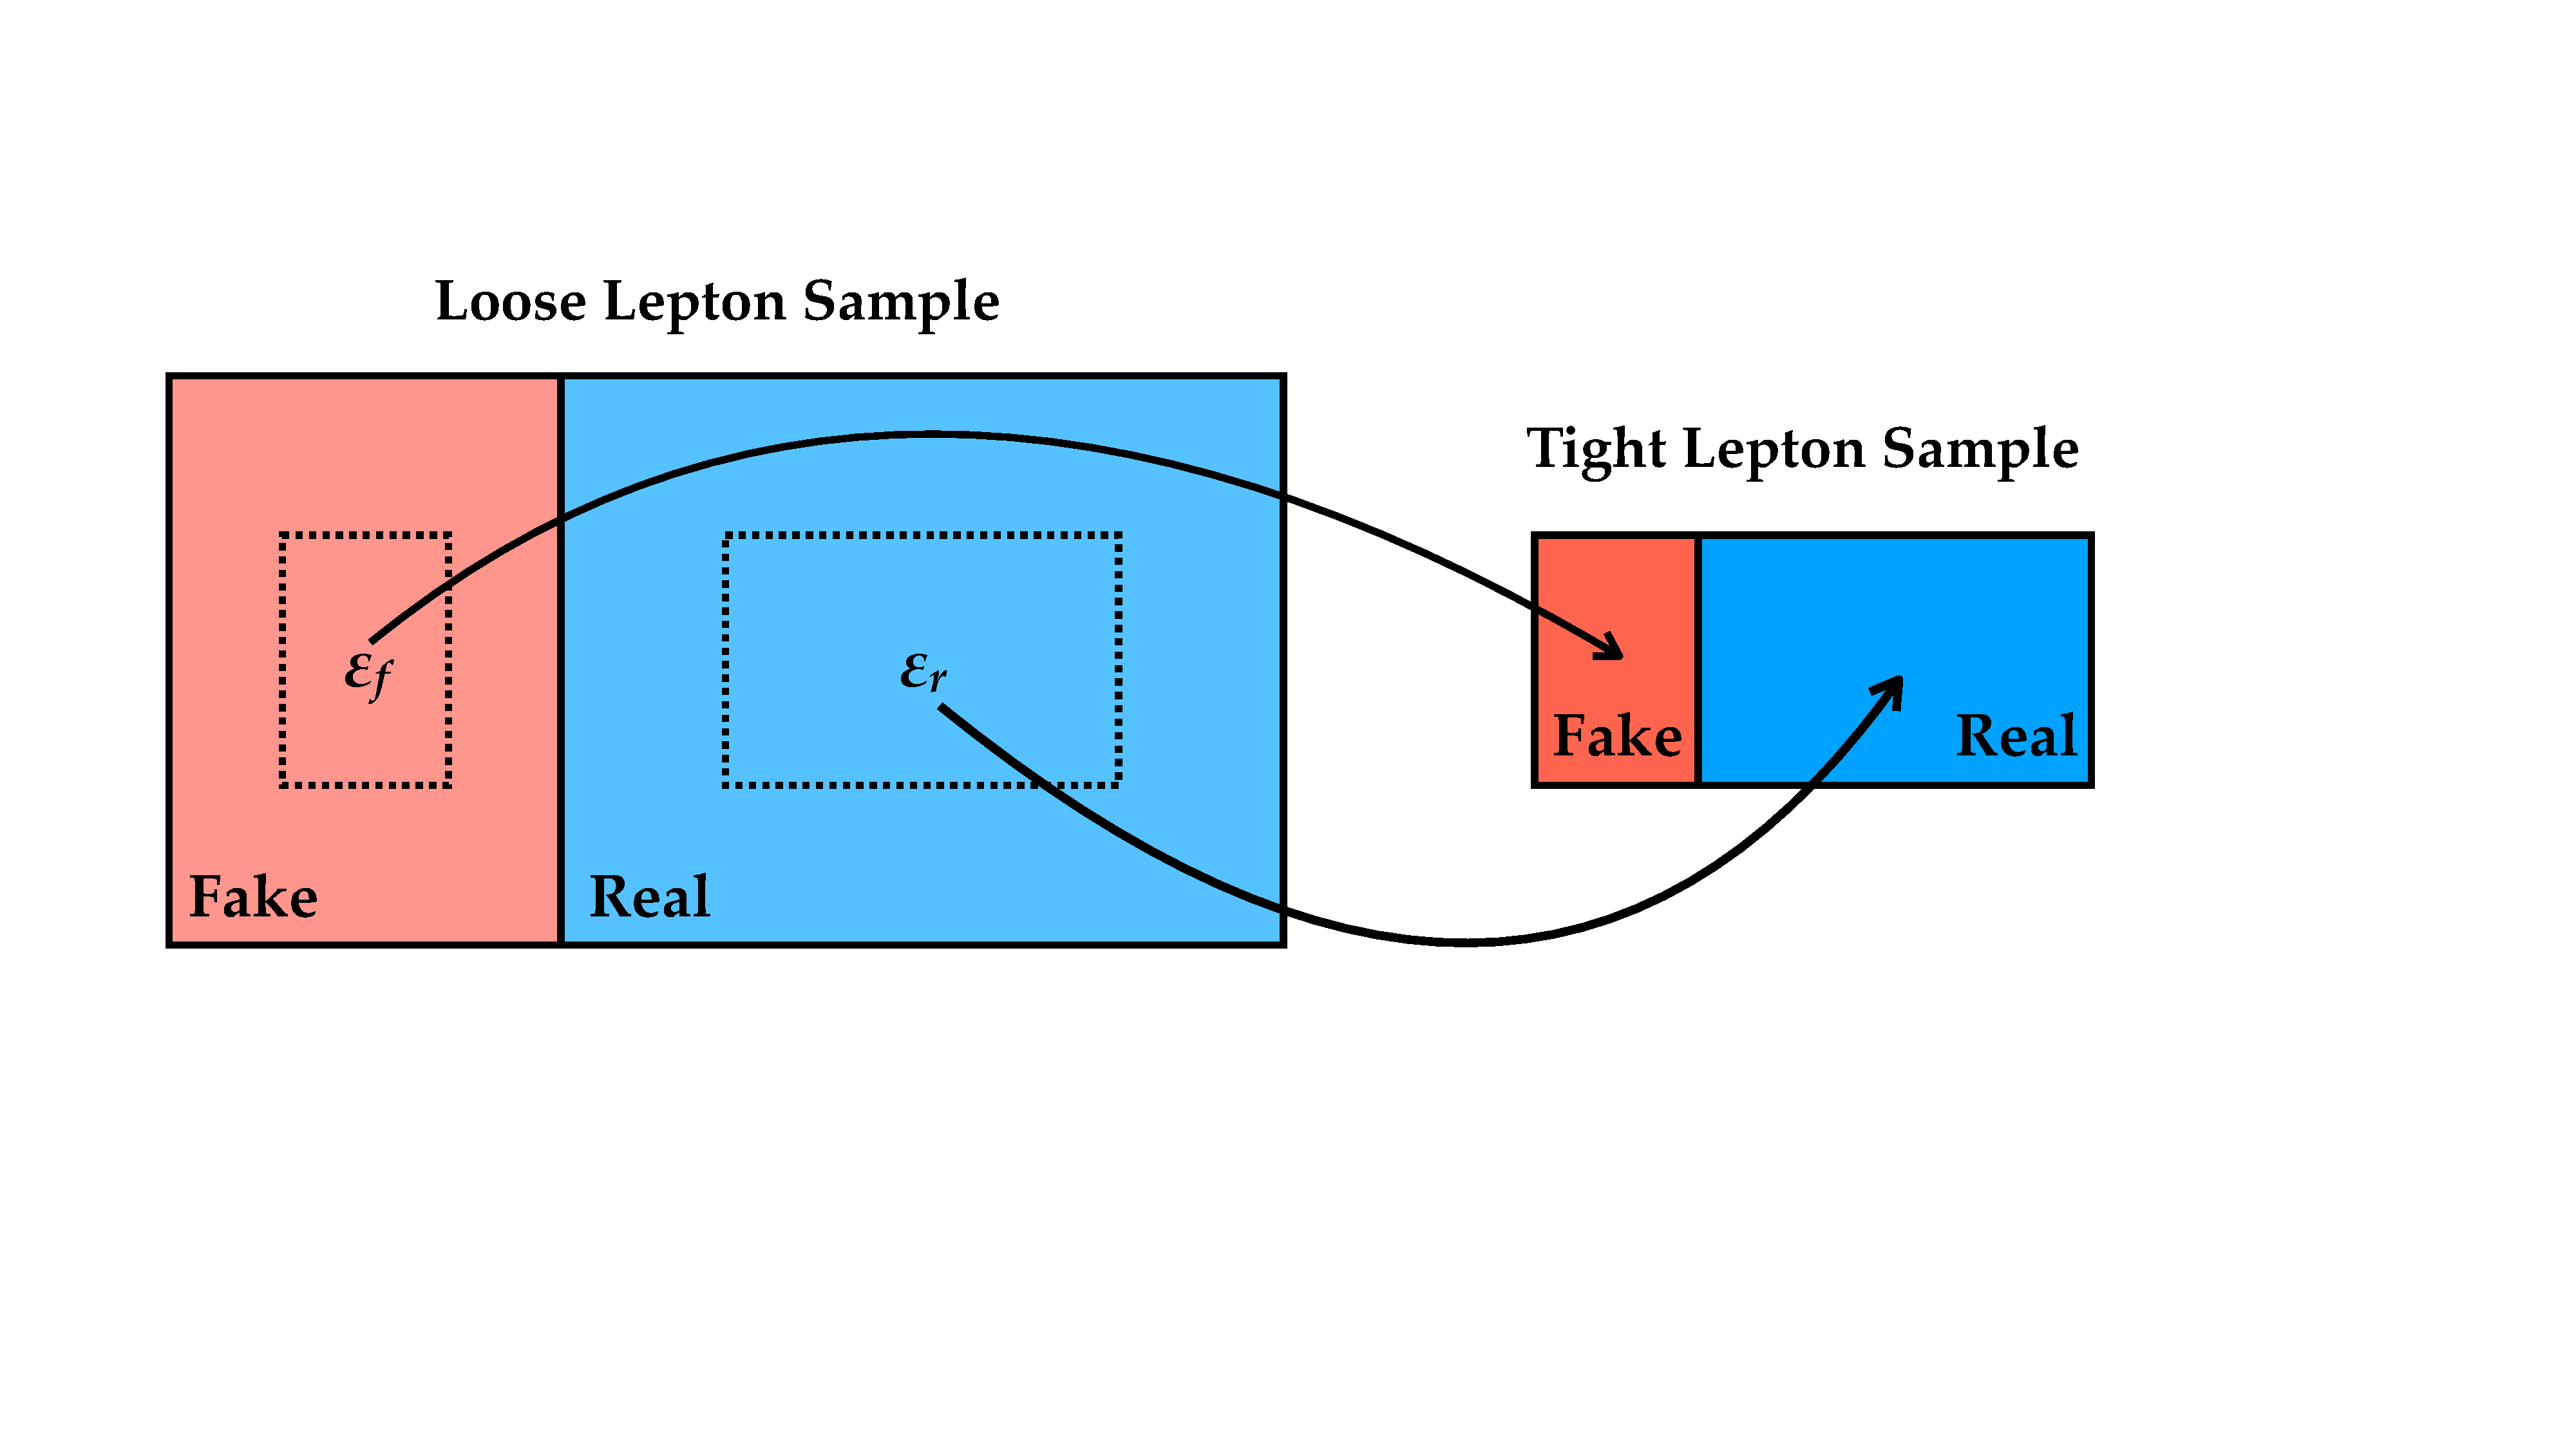
\includegraphics[width=0.65\textwidth]{figures/common_ana/fakes/fake_effs_illustration}
        \caption{
        }
        \label{fig:fake_effs}
    \end{center}
\end{figure}

The real efficiencies, $\varepsilon_r$, are measured in data using $Z$-boson tag-and-probe methods, requiring the probe lepton
to satisfy the Tight lepton selection and to be matched to the trigger.
The probe lepton must satisfy the Loose lepton selection.
The fraction of loose probe leptons to pass the Tight lepton selection then gives a measure of $\varepsilon_r$.

The fake efficiencies, $\varepsilon_f$, are measured in data using events with different-flavor leptons,
where one lepton is an electron and the other is a muon, that have the same electric charge.
A tag-and-probe method similar to that used in the measurement of $\varepsilon_r$ is used
and relies on the fact that a comparatively small amount of SM processes can result in same-sign
and different-flavor events.
Therefore, when a probe satisfies the Tight selection it is very likely to be the case that the
probe lepton is a fake lepton.
An additional component of the $\varepsilon_f$ is measured by additionally requesting that there
be at least one $b$-tagged jet in the same-sign, different-flavor selection.
This allows for $\varepsilon_f$ to be measured in a region enriched in fake leptons originating
from semi-leptonic decays of heavy-flavor jets.
The various measurements of $\varepsilon_f$ are combined following an averaging scheme, weighted according
to the composition of fake lepton sources expected to contaminate the SRs.

The real and fake efficiencies are not global quantities.
Instead, they are measured as a function of both the lepton $\pT$ and $\eta$
such that they may track the effects of changes in detector response and
material interaction over the $\pT$ and $\eta$ ranges relevant to the leptons used in the analysis.

Once $\varepsilon_r$ and $\varepsilon_f$ are obtained, the fake lepton background
can be obtained by inverting the equation relating the measured quantities (Tight versus Loose), taken
from the observed data, in terms
of those that we want to know (Fake versus Real):
\begin{equation}
    \begin{pmatrix}
        N_{TT} \\ N_{TL} \\ N_{LT} \\ N_{LL}
    \end{pmatrix}
        = M
    \begin{pmatrix}
        N_{LL}^{RR} \\ N_{LL}^{RF} \\ N_{LL}^{FR} \\ N_{LL}^{FF}
    \end{pmatrix}
    \label{eq:matrix_method}
\end{equation}
\noindent where in the sub- and super-scripts, the first (second) index refers to the leading (sub-leading) lepton.
The sub-script `$T$' (`$L$') refers to the lepton passing the Tight (Loose) lepton
selection.
The super-script `$R$' (`$F$') indicates whether or not the lepton is a real (fake) lepton.
For example, the quantity $N_{LL}^{FR}$ is the number of events in which the leading lepton
in the sample of Loose leptons is fake and the sub-leading is real.
The matrix $M$ is given by,
\begin{align}
    M = \begin{pmatrix}
            r_1 r_2 & r_1 f_2  & f_1 r_2 & f_1 f_2 \\
            r_1 \overline{r_2} & r_1\overline{f_2} & f_1 \overline{r_2} & f_1 \overline{f_2} \\
            \overline{r_1} r_2 & \overline{r_1} f_2 & \overline{f_1} r_2 & \overline{f_1} f_2 \\
            \overline{r_1} \overline{r_2} & \overline{r_1} \overline{f_2} & \overline{f_1} \overline{r_2} & \overline{f_1} \overline{f_2}
        \end{pmatrix}
    \label{eq:matrix_method_matrix}
\end{align}
where $r_i$ ($f_i$) is shorthand for the real (fake) efficiency, $\varepsilon_r$ ($\varepsilon_f$),
and the notation $\overline{x_i}$ indicates $(1 - x_i)$.
%To make clear the data-driven aspect of the method:
%both sets of qauntities --- those appearing on the left-hand-side of Equation~\ref{eq:matrix_method} and the $r_i$ and $f_i$ ---
%are measured using the observed data.

The number of events with double-fake and single-fake leptons satisfying the analysis' Tight selection
($N_{TT}^{FF}$ and $N_{TT}^{RF} + N_{TT}^{FR}$, respectively) can then be obtained from the
number of events with double-fake and single-fake leptons satisfying the Loose selection
($N_{LL}^{FF}$ and $N_{LL}^{RF} + N_{LL}^{FR}$, respectively) through inversion
of Equation~\ref{eq:matrix_method}  and
noting the following relations,
\begin{align}
    N_{TT}^{RR} &= r_1 r_2 \cdot N_{LL}^{RR}  \label{eq:matrix_method_sol0}\\
    N_{TT}^{RF} &= r_1 f_2 \cdot N_{LL}^{RF}  \label{eq:matrix_method_sol1}\\
    N_{TT}^{FR} &= f_1 r_2 \cdot N_{LL}^{FR}  \label{eq:matrix_method_sol2}\\
    N_{TT}^{FF} &= f_1 f_2 \cdot N_{LL}^{FF}. \label{eq:matrix_method_sol3}
\end{align}
The quantities appearing on the right-hand-side of Equations~\ref{eq:matrix_method_sol0}-\ref{eq:matrix_method_sol3}
depend entirely on the observed data.
The number of events in the analysis' Tight selection that have at least one fake lepton is then given by the sum
$N_{TT}^{RF} + N_{TT}^{FR} + N_{TT}^{FF}$.
This gives a total integrated yield for the fake background contribution in the analysis'
Tight selection; however, from Equations~\ref{eq:matrix_method_sol1}-\ref{eq:matrix_method_sol3}
a set of per-event weighting factors (`fake weights'), depending only on the $\varepsilon_r(\pT,\eta)$ and
$\varepsilon_f(\pT,\eta)$ efficiency factors for the two leptons, can be defined.
These fake weights allow for kinematic distributions of the fake lepton background
sources to be populated
by appropriately applying them to events in the data sample consisting of leptons satisfying the analysis' Loose selection.



%%%%%%%%%%%%%%%%%%%%%%%%%%%%%%%%%%%%%%%%%%%%%%%%%%%%%%%%%%%%%%%%%%%
%%%%%%%%%%%%%%%%%%%%%%%%%%%%%%%%%%%%%%%%%%%%%%%%%%%%%%%%%%%%%%%%%%%
%
% SAME SIGN EXTRAPOLATION
%
%%%%%%%%%%%%%%%%%%%%%%%%%%%%%%%%%%%%%%%%%%%%%%%%%%%%%%%%%%%%%%%%%%%
%%%%%%%%%%%%%%%%%%%%%%%%%%%%%%%%%%%%%%%%%%%%%%%%%%%%%%%%%%%%%%%%%%%
\subsection{Same-sign Extrapolation Method}
\label{sec:same_sign_extrap}

The Same-sign Extrapolation Method is another method for
estimating the numbers of events with fake and non-prompt leptons.
This method is well described in Refs.~\cite{TOPQ-2015-09,TOPQ-2017-05}.
The method is tailored for dilepton analyses that require the two
leptons to have opposite electric charge and takes advantage of the fact that the
production mechanisms for the fake leptons described above are generally
uncorrelated with the charges of leptons in the event.
This means that the rates of the various sources of fake leptons will generally
be the same in the sample of oppositely-charged dilepton events and in the
sample of dilepton events in which the leptons have the same charge.
The former are referred to as opposite-sign (OS) events and the latter
as same-sign (SS) events.
This assumption is not entirely correct, however, since the underlying sources of
the fake and/or non-prompt leptons are not all charge symmetric.\footnote{`Charge-symmetric' means that the
dilepton final state of a given process may be either OS or SS, with equal probability of each case occuring.}
For example, a dominant source of mis-identified leptons in dileptonic events
arises from the production of semi-leptonically decaying top-quark pairs, in which the sub-leading reconstructed
electrons arise from a mis-identified jet.
This process is charge-symmetric since
converted photons produced in jets are equally likely to give rise to a reconstructed
$e^+$ or $e^-$ and are uncorrelated to the sign of the real lepton.
In trident decays whereby bremsstrahlung photons (radiated from the lepton children
of the top-quarks) undergo conversion processes, however, there is a partial
charge correlation of the reconstructed electron with the charge of the original lepton,
and hence a larger contribution to the OS sample of events.
These two cases are illustrated in Figure~\ref{fig:ttbar_fake_charge_sym}.
The lepton definitions within the OS and SS event samples are the same.
That is, they use the same reconstruction, identification, and isolation working points.
This is compared to the Matrix Method, in which the two samples of leptons used in the technique's
implementation differ by their lepton definitions.

\begin{figure}[!htb]
    \begin{center}
        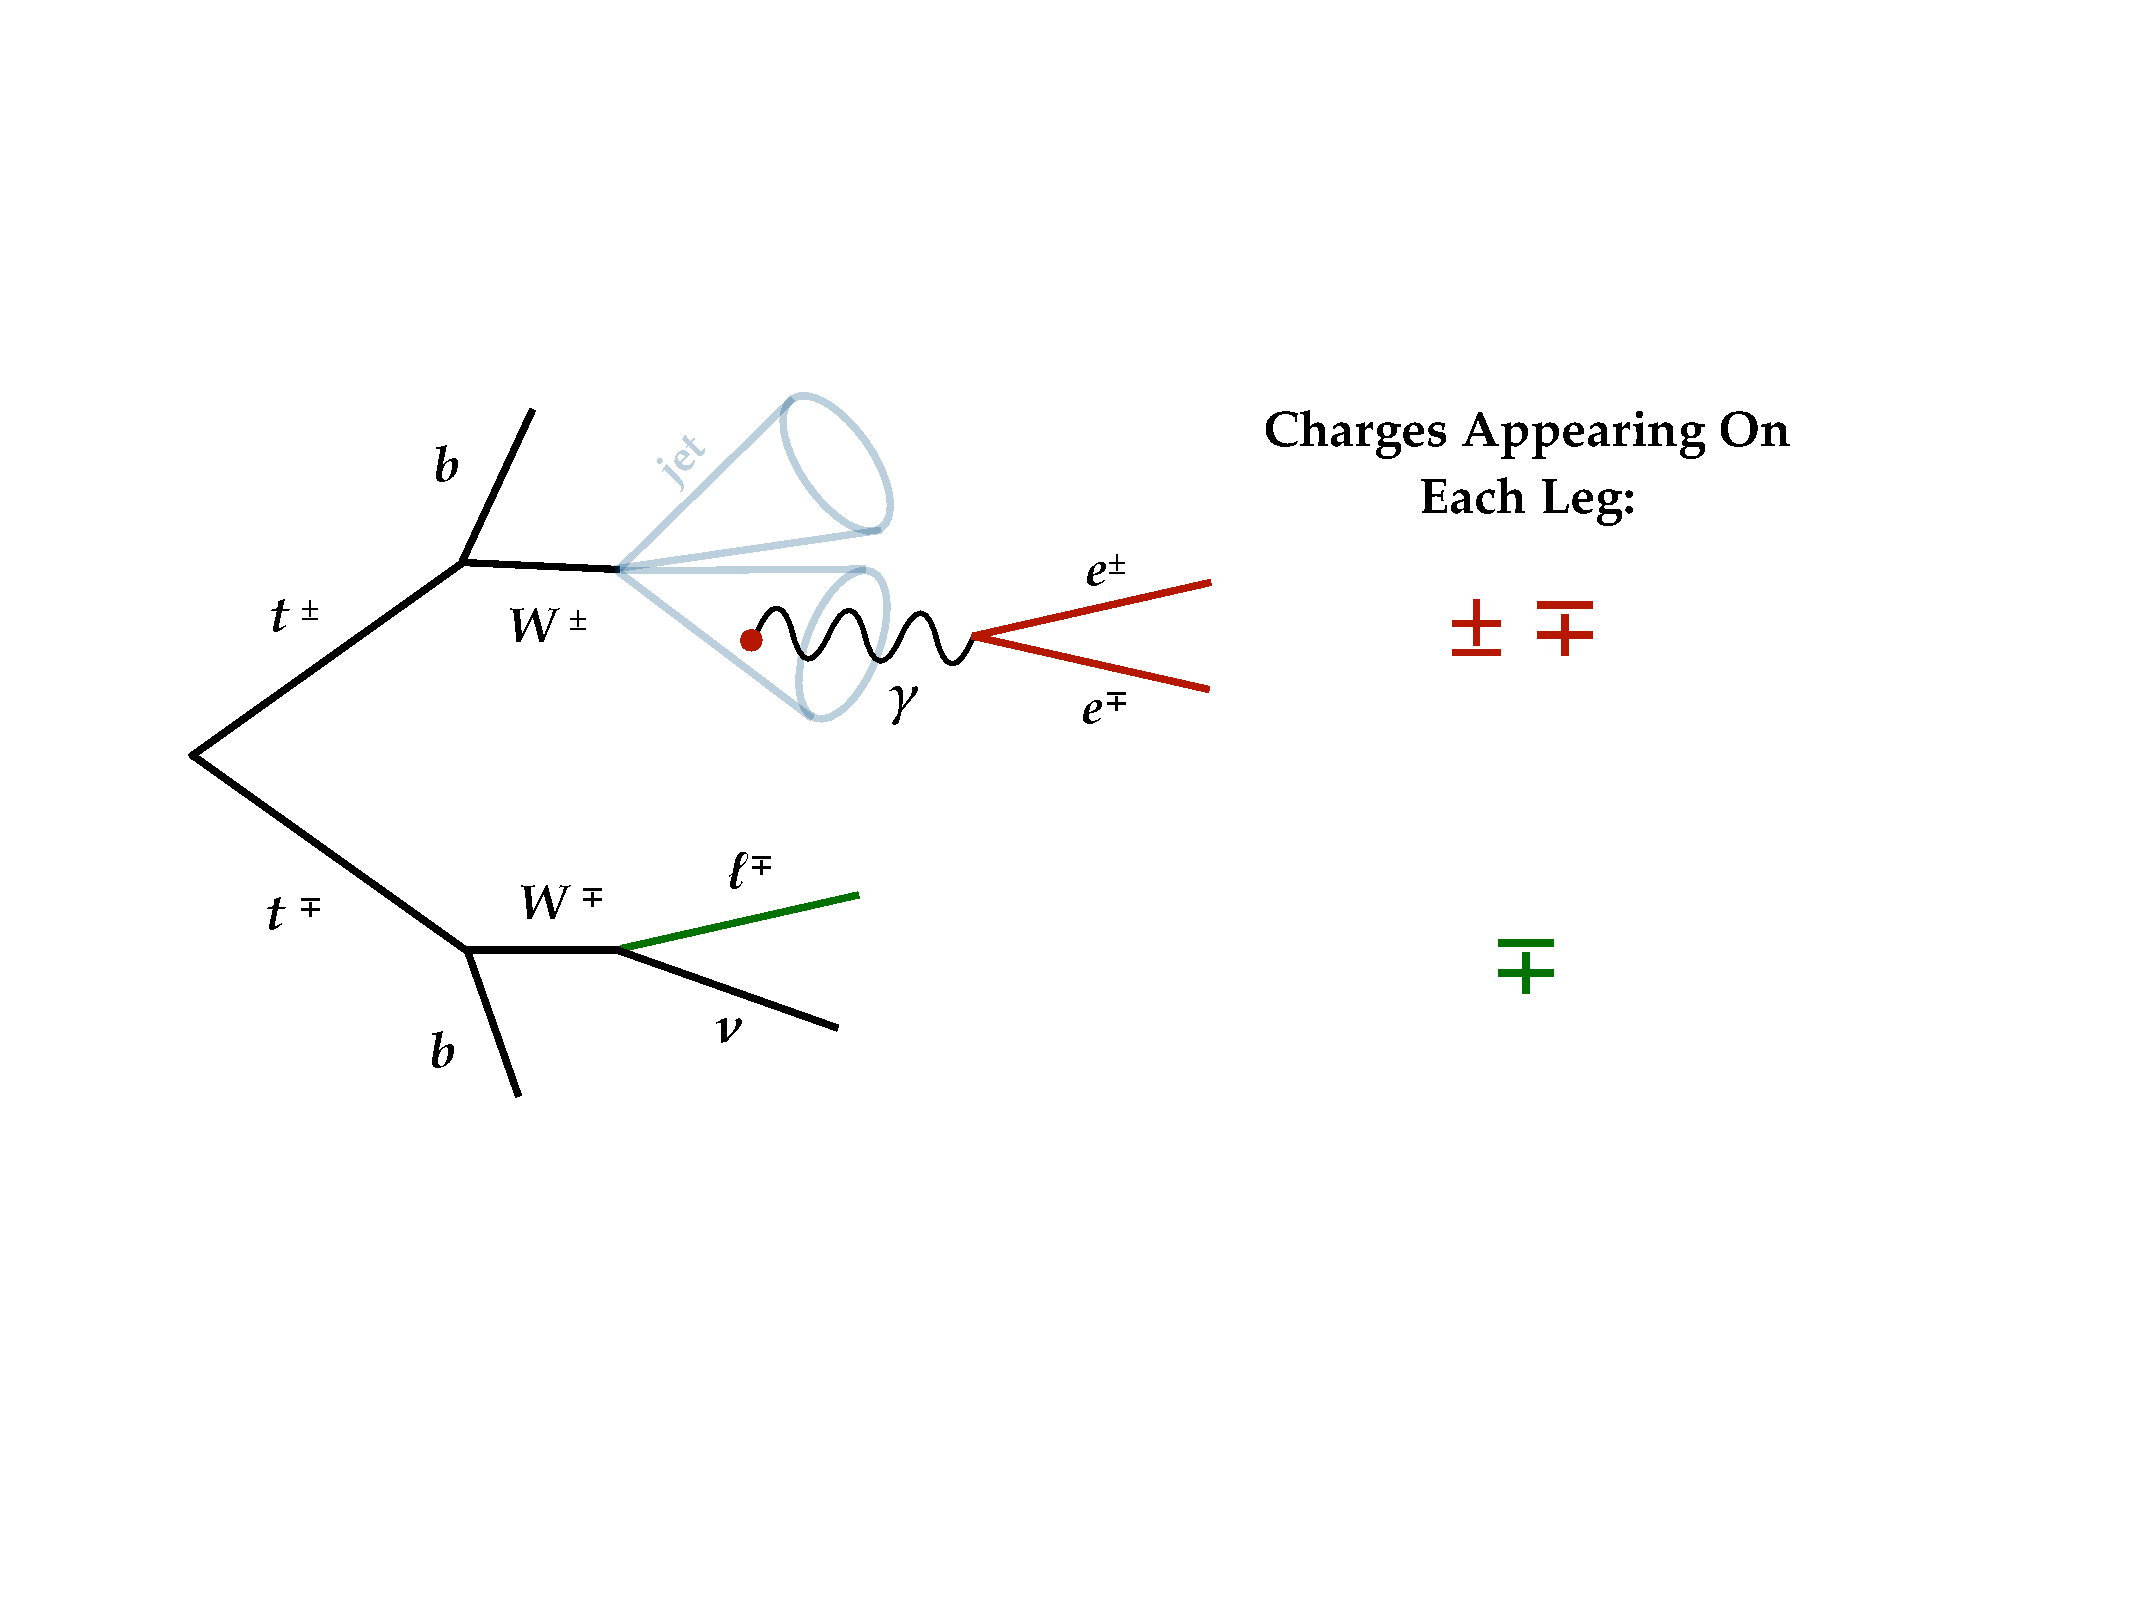
\includegraphics[width=0.7\textwidth]{figures/common_ana/fakes/ttbar_fake_charge_sym_semi}
        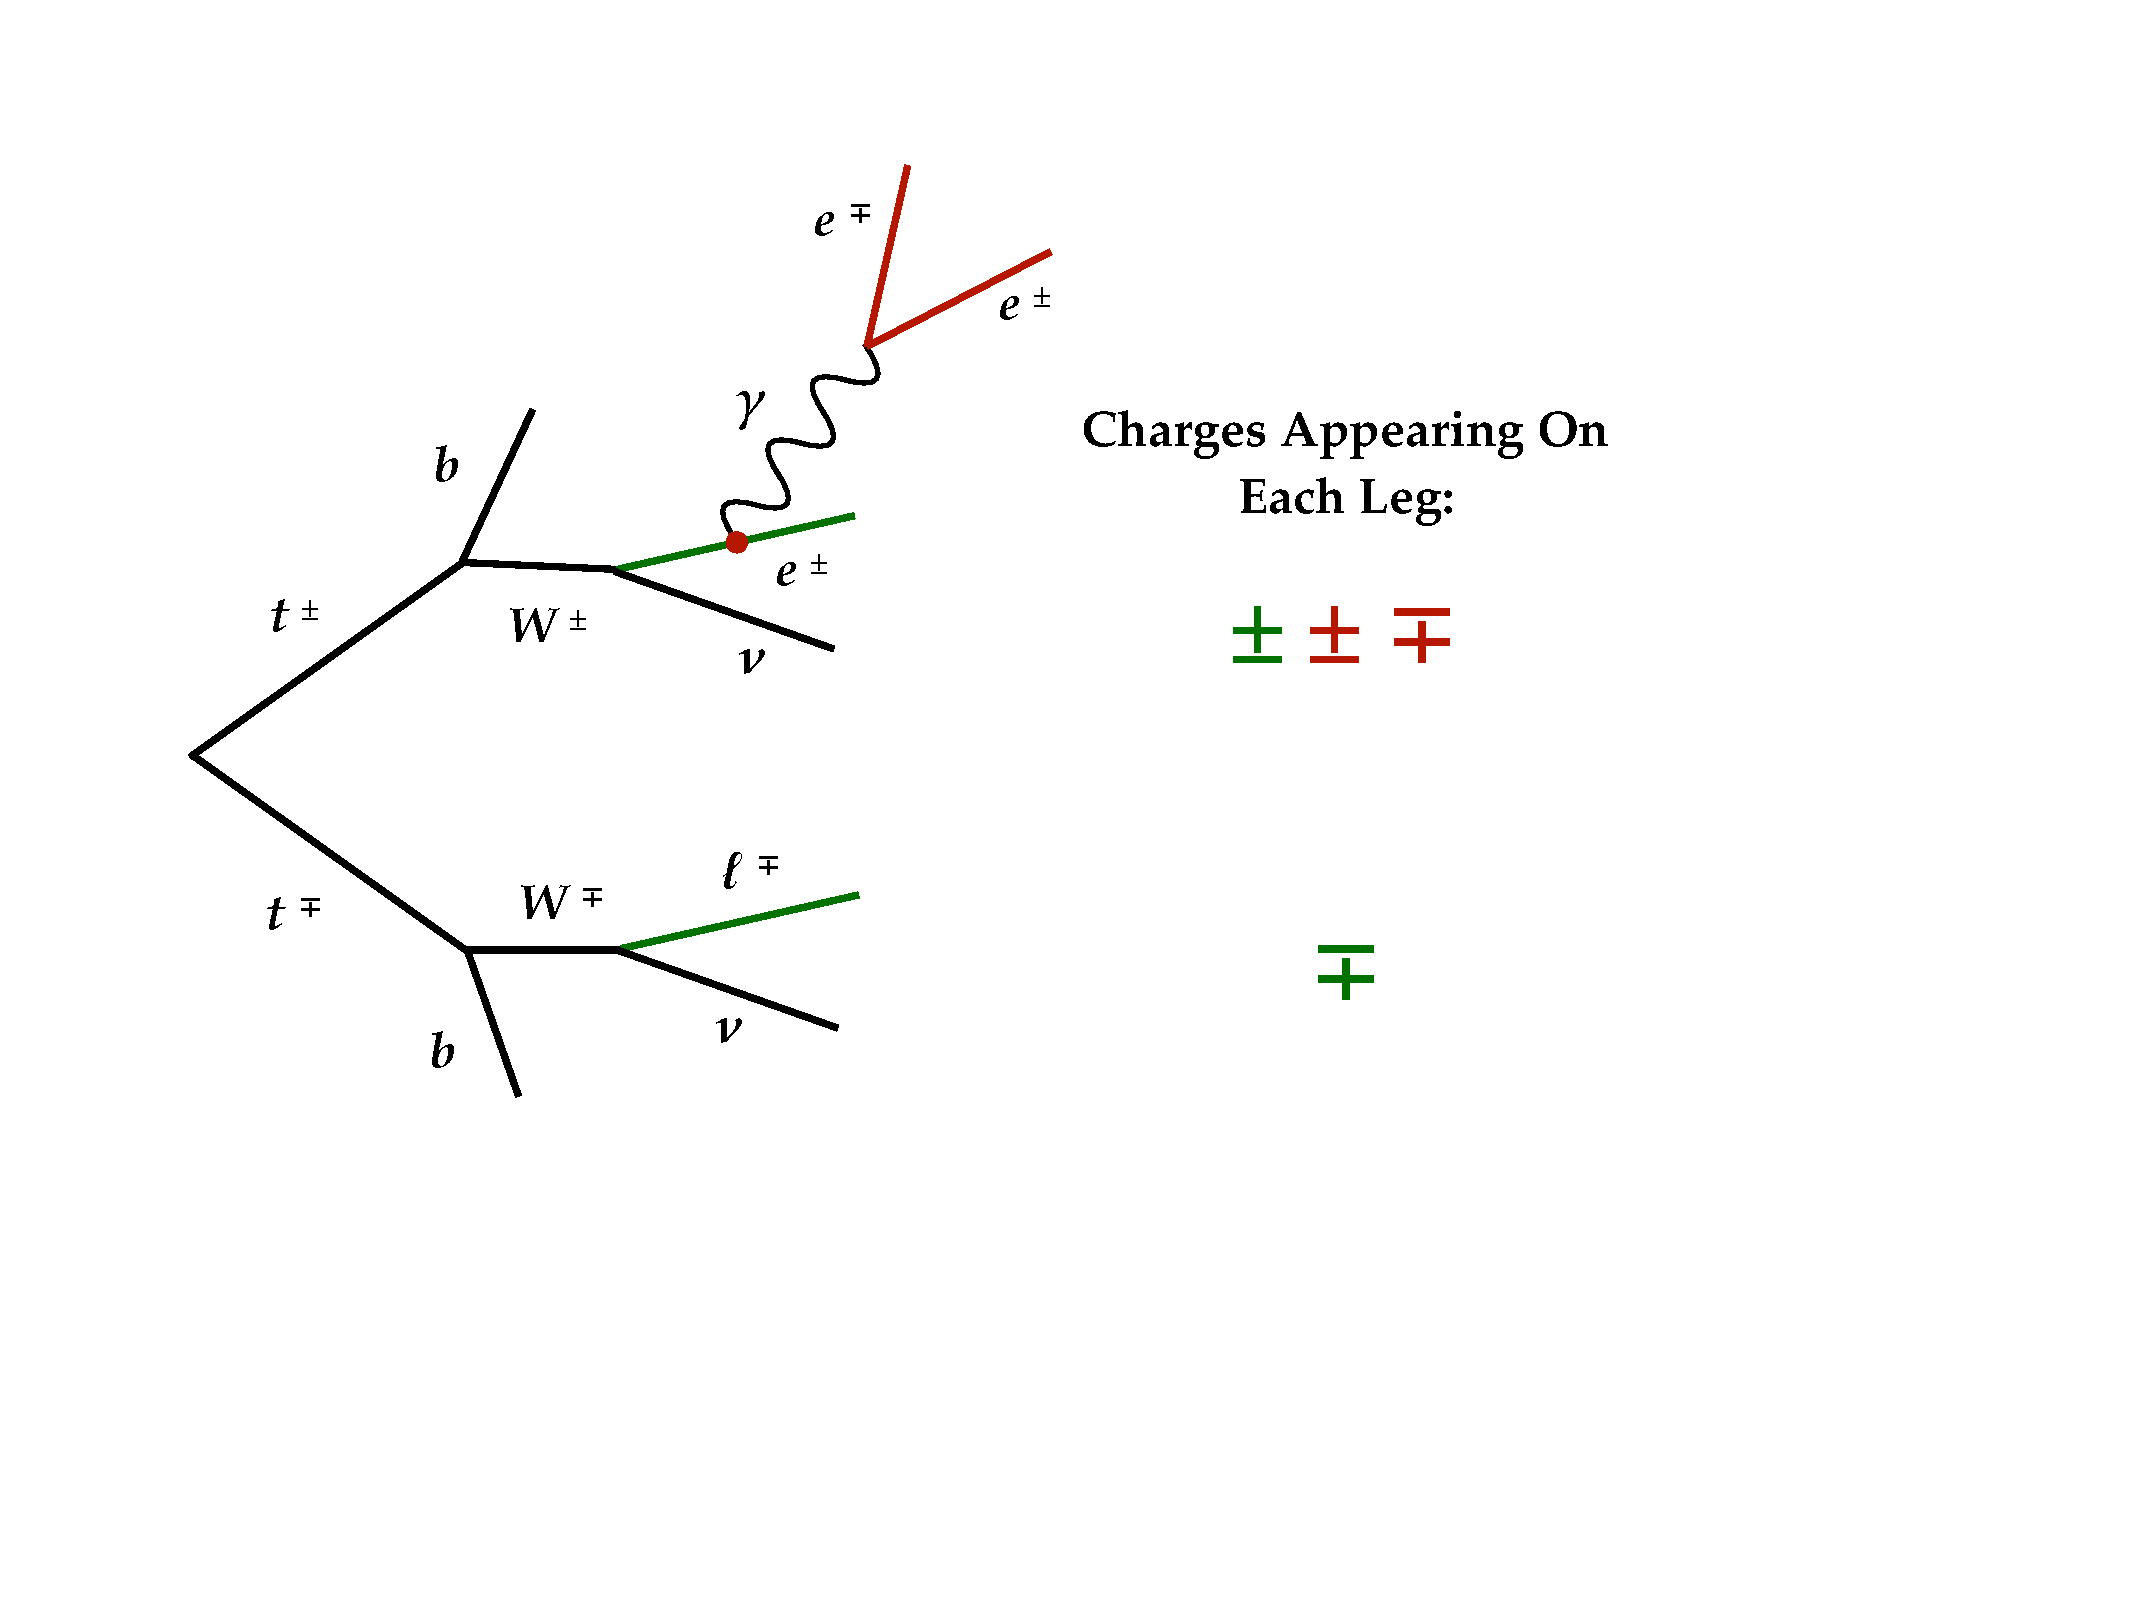
\includegraphics[width=0.7\textwidth]{figures/common_ana/fakes/ttbar_fake_charge_sym_trident}
        \caption{
            Illustration of charge-asymmetry in fake lepton production
            arising in top-quark pair production events, leading to
            the rate of photon conversion sources of fake electrons being larger in OS dilepton events.
            \textbf{\textit{Top}}: Shower photons arising from decays within one of the jets
                in semi-leptonic decays of top-quark pairs may convert to an electron-positron pair,
                leading to one of the jets being reconstructed as an electron.
                Looking at the charge possibilities of each side of the top-quark pair decay,
                the event is equally likely to be classified as either an OS or SS event.
            \textbf{\textit{Bottom}}: Trident events arising in dileptonic top-quark pair production
                events can lead to a non-prompt electron from the photon conversion being selected
                as one of the event's candidate leptons.
                The overall charge possibilites of the lepton charges on the side of the trident decay
                are correlated with the charge of the initial lepton.
                Looking at the charge combinations possible between both sides of the top-quark pair decay,
                the event is more likely to be classified as an OS event.
        }
        \label{fig:ttbar_fake_charge_sym}
    \end{center}
\end{figure}

The method also assumes that the rate of dilepton events in which \textit{both} leptons
are fake is negligible, and that the composition of the fake background contributing to
the dilepton final state is composed of events in which one of the leptons is real.
In the majority of cases, the sub-leading lepton is the fake lepton.
For this reason, when using the MC simulation to gain predictions of the composition of
the fake backgrounds, the MC events in which only one of the leptons is fake are considered.
This will become clear in the discussion to follow and in the specific implementation described
in Chapter~\ref{chap:search_hh}.


The general method works as follows.
Since, as described above, the rates of the various sources of fake backgrounds in the OS and SS samples of events
are generally the same, the method relies on using the sample of SS events to provide a template of the fake backgrounds
to be used in the OS selections.
The contribution of fakes to each of the regions (CR, VR, or SR) in the analysis is estimated
by subtracting the prediction of the prompt (real) SM backgrounds from the observed data
in the associated SS selections, defined similarly to the OS selections used in the analysis but with the
charge-requirements inverted.
The ratio of the number of OS to SS events with fake leptons, $f^{SS \rightarrow OS}$,
is taken entirely from MC and is applied to the SS data that has had the prompt-MC contribution
subtracted in order to extrapolate this number to the OS regions.
This SS extrapolation is described by Equation~\ref{eq:ss_extrap}.

\begin{align}
    N_{\text{OS}}^{\text{fake}} &= f^{SS \rightarrow OS} \times N_{\text{SS}}^{\text{fake}} \nonumber \\
        &= \frac{ N_{\text{MC,OS}}^{\text{fake}} }{ N_{\text{MC,SS}}^{\text{fake}} } \times ( N_{\text{data,SS}} - N_{\text{MC,SS}}^{\text{real}} )
        \label{eq:ss_extrap}
\end{align}

In addition to providing overall yields fake backgrounds in a given region,
the method described by Equation~\ref{eq:ss_extrap} provides the means to
inspect the kinematics of the predicted fake backgrounds by simply computing
Equation~\ref{eq:ss_extrap} on a bin-by-bin basis when populating histograms
of kinematic observables.

Further details on the implementation of the Same-sign Extrapolation Method,
described by Equation~\ref{eq:ss_extrap}, will be given in Chapter~\ref{chap:search_hh}.
In particular, the implicit sensitivities to the MC simulation will be described,
as well as additional extrapolations specific to the analysis.
